\begin{figure*}[ht]
\centering
\begin{minipage}{0.9\textwidth}
\centering
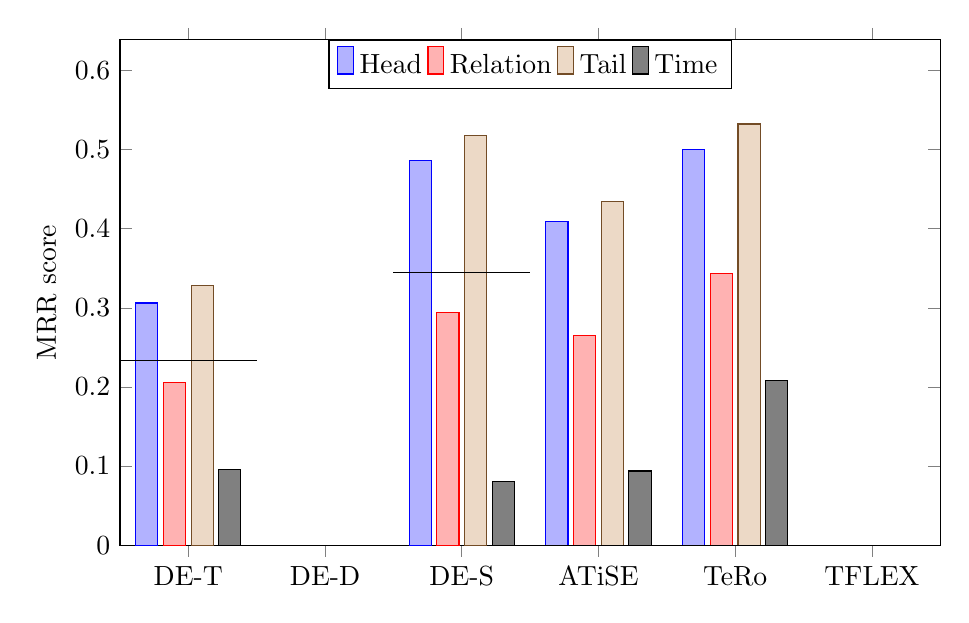
\begin{tikzpicture}
\begin{axis}[
    ybar,
    bar width=8pt,
    xticklabels={x,DE-T,DE-D,DE-S,ATiSE,TeRo,TFLEX},
    ymin=0,
    ymax=0.6387472890106644,
    ylabel={MRR score},
    height=8cm,
    width=12cm,
    legend style={
        at={(0.5,1.0)},
        anchor=north,
        legend columns=-1
    },
    legend image code/.code={
        \draw [#1] (0cm,-0.1cm) rectangle (0.2cm,0.25cm); },
    ]
\addplot coordinates { %head
(0, 0.3060130826437023) %DE_TransE
(1, 0) %DE_DistMult
(2, 0.485840495935422) %DE_SimplE
(3, 0.40864722143311377) %ATISE
(4, 0.4998850216977859) %TERO
(5, 0) %TFLEX
} ;
\addplot coordinates { %relation
(0, 0.2050733839712357) %DE_TransE
(1, 0) %DE_DistMult
(2, 0.29419180983873955) %DE_SimplE
(3, 0.2651920008232943) %ATISE
(4, 0.34365312580396906) %TERO
(5, 0) %TFLEX
} ;
\addplot coordinates { %tail
(0, 0.3277892854794874) %DE_TransE
(1, 0) %DE_DistMult
(2, 0.5174294134375389) %DE_SimplE
(3, 0.4339695690436387) %ATISE
(4, 0.532289407508887) %TERO
(5, 0) %TFLEX
} ;
\addplot coordinates { %time_from
(0, 0.09517766038307589) %DE_TransE
(1, 0) %DE_DistMult
(2, 0.0809454461243896) %DE_SimplE
(3, 0.09372231337334733) %ATISE
(4, 0.20829942435104987) %TERO
(5, 0) %TFLEX
} ;
\addplot[black,sharp plot,update limits=false,] coordinates { %DE_TransE
(-0.5, 0.23351335311939853)
(0.5, 0.23351335311939853)
} ;
\addplot[black,sharp plot,update limits=false,] coordinates { %DE_DistMult
(0.5, 0)
(1.5, 0)
} ;
\addplot[black,sharp plot,update limits=false,] coordinates { %DE_SimplE
(1.5, 0.3446017913340443)
(2.5, 0.3446017913340443)
} ;
\addplot[black,sharp plot,update limits=false,] coordinates { %ATISE
(2.5, 0)
(3.5, 0)
} ;
\addplot[black,sharp plot,update limits=false,] coordinates { %TERO
(3.5, 0)
(4.5, 0)
} ;
\addplot[black,sharp plot,update limits=false,] coordinates { %TFLEX
(4.5, 0)
(5.5, 0)
} ;
\legend{Head,Relation,Tail,Time}
\end{axis}
\end{tikzpicture}
\caption{icews14, split 1}
\label{fig:compare_icews14_1}
\end{minipage}
\end{figure*}
